\chapter{RC filters}

\section*{AIM}
\paragraph{}To design and implement circuits for passive RC highpass and lowpass filters.

\section*{DESIGN AND CIRCUIT DIAGRAM}
\paragraph{}

Inorder to plot the frequency response of RC highpass and lowpass filters use an AC source whose frequency can be varied durinmg simulation. The AC source is connected across a series connection of resistor and capacitor. The corresponding circuits for RC highpass filter and lowpass filters are shown in figures \ref{rchpf} and  \ref{rclpf} respectively. The cutoff frequency of the filter will be given by \begin{equation}
f_c=\frac{1}{2\pi RC}
\end{equation}

\begin{figure}[h]
\centering
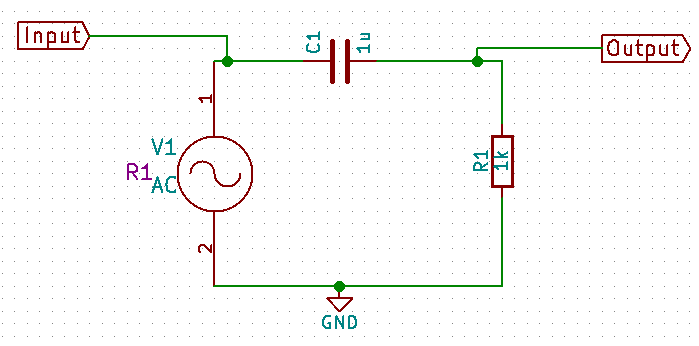
\includegraphics[width=0.8\textwidth]{rchpf.png}
\caption{Schematic diagram for passive RC high pass filter}
\label{rchpf}
\end{figure}

\begin{figure}[h]
\centering
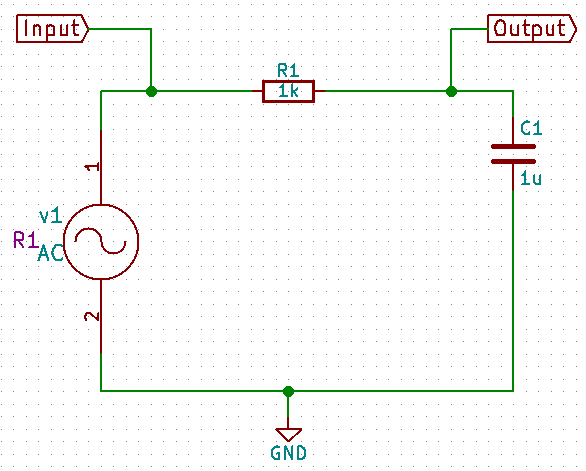
\includegraphics[width=0.8\textwidth]{rclpf.png}
\caption{Schematic diagram for passive RC low pass filter}
\label{rclpf}
\end{figure}

\section*{PROCEDURE}

\paragraph{}Explained below are the steps to plot the characteristics of RC high pass filter. Follow the same procedure to obtain the response of RC lowpass filter (Set the project name as RC\_LPF and draw the schematic as shown in figure \ref{rclpf}.)


\subsection{Launch eSim}

\paragraph{}
 Launching eSim will take you to the dialog box which asks for the default workspace. Browse the folders and set the wokspace location. It will finally end up in the eSim window shown in Figure \ref{LaunchWindow}.
\begin{figure}[h]
\centering
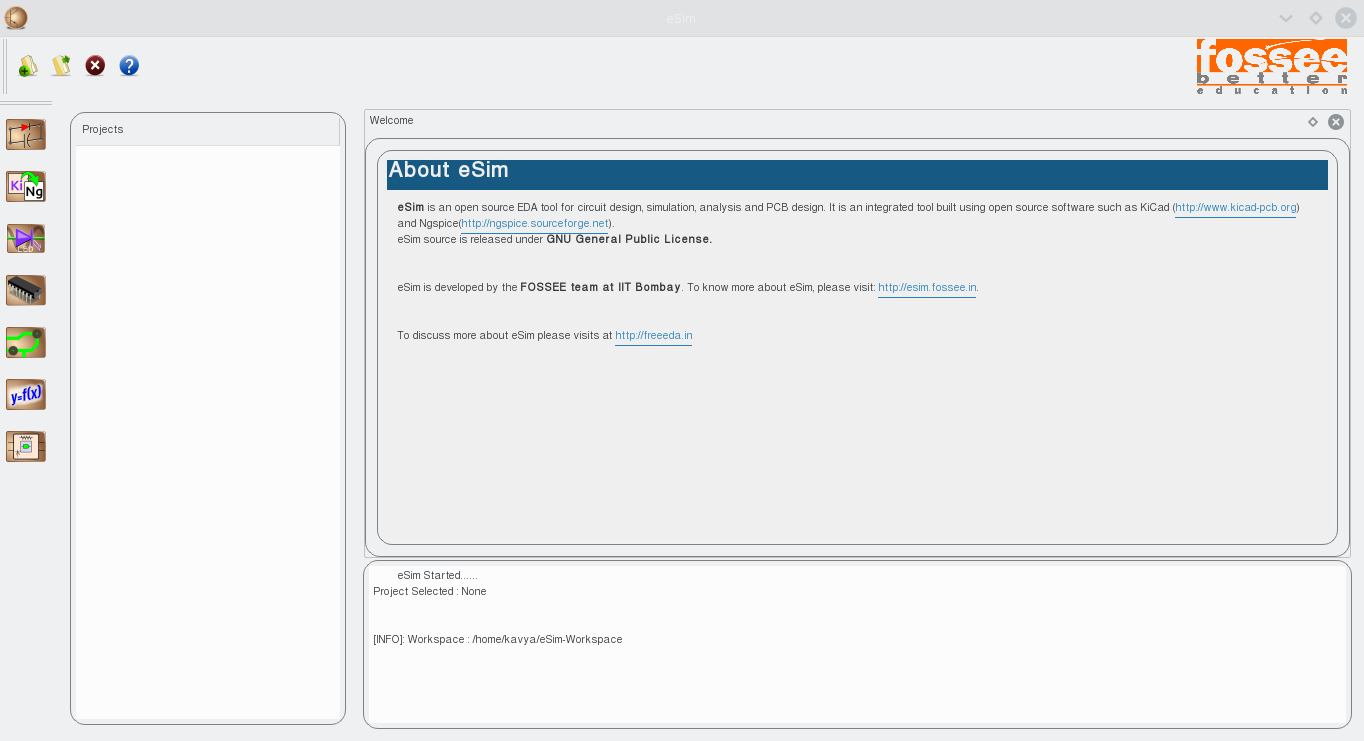
\includegraphics[width=0.8\textwidth]{LaunchWindow.png}
\caption{Launching eSim will take you to this window}
\label{LaunchWindow}
\end{figure}

\subsection{Create a New Project}

\paragraph{ } The new project is created by clicking the New icon on the
menubar. The name of the project is given in the pop up window as RC\_HPF for highpass filter.
\subsection{Create the Schematic}

\paragraph{}  To create the schematic, click the very first icon of the
left toolbar. This will open KiCad Eeschema.


To create a schematic in KiCad, we need to place the required components. After all the required components of the simple RC circuit are placed, wiring is
done using the Place Wire option. The `Place Wire' and `Place Component' tools are available in the left toolbar. Scroll up and down for zooming in and out.


%\begin{figure}
%\begin{minipage}{.5\textwidth}
%  \centering
%  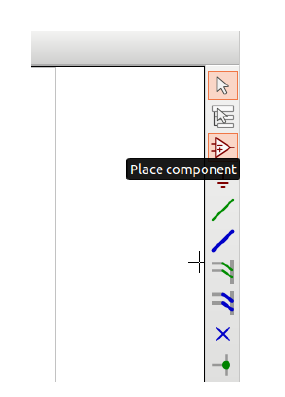
\includegraphics[width=\linewidth]{placecomponent.png}
%  \caption{Place component icon}
%  \label{placecomponent}
%\end{minipage}%
%\begin{minipage}{.5\textwidth}
%  \centering
%  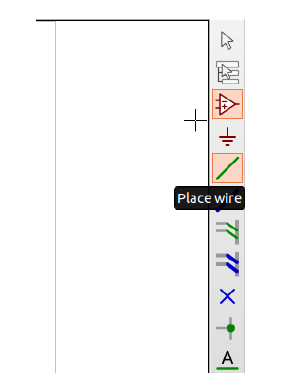
\includegraphics[width=\linewidth]{placewire.png}
%  \caption{Place wire icon}
%  \label{placewire}
%\end{minipage}
%\end{figure}


\paragraph{Placing the Components:} Normally all the components availbale in eSim can be chosen by left mouse click in the grid. The components are listed in different libraries. See Figure \ref{librarylist}.

\begin{figure}[h]
\centering
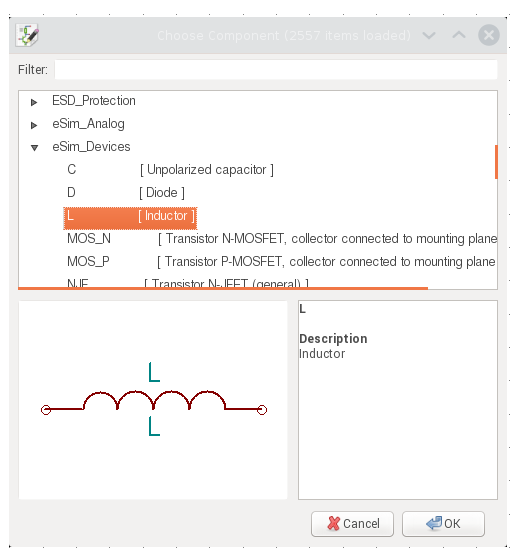
\includegraphics[width=0.5\textwidth, height=4cm]{librarylist.png}
\caption{The Kicad Libraries of components}
\label{librarylist}
\end{figure}

\begin{itemize}
\item
Choose AC source from eSim\_Sources
\item
Choose R from eSim\_Devices
\item
Choose C from eSim\_Devices
\item
Choose GND from power
\end{itemize}

Select the resistor and edit its component value to 1k as shown in Figure \ref{editvalue}. Also edit the value of capacitor as 1 $\mu$ F. You can just type in 1u.

\begin{figure}[h]
\centering
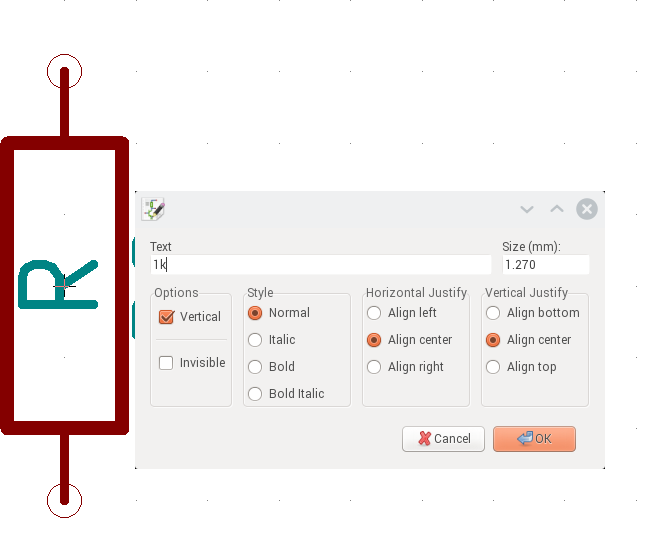
\includegraphics[width=0.5\textwidth, height=6cm]{editvalue.png}
\caption{Editing the value field of component R}
\label{editvalue}
\end{figure}

Wire the components to get the circuit. A global label `Input'  and `Output' has been added to identify that node whose voltage will be later recorded and plotted. Global label is added from the right toolbar of Eeschema.

\paragraph{Annotating the circuit:} Once the schematic diagram is completed, annotate it so that the `question marks' associated with the components are converted to meaningful numbers automatically.For that choose annotate button from the top toolbar(See Figure \ref{toptoolbar} and in the subsequenct dialogue boxes appearing click ok and finally close. See Figure \ref{annotation}.

\begin{figure}[h]
\centering
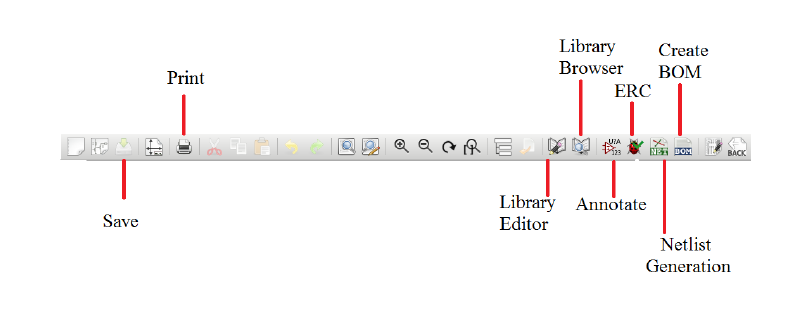
\includegraphics[width=\textwidth, height=4cm]{toptoolbar.png}
\caption{Choose annotate from the toop tool bar}
\label{toptoolbar}
\end{figure}



Now we have the circuit diagram as shown in Figure \ref{rchpf}.


\paragraph{Note:} If some libraries are found missing, you can add them from the `Preferences` menu by following the procedure: 

\begin{enumerate}
\item
Choose `Component Libraries' from Preferences menu.

\item
Click on the Add button on the top right side of the window.

\item
Choose the required libraries from `user/share/kicad/library' and click OK button

\end{enumerate}

\subsection{Create Netlist}

\paragraph{}To simulate the circuit that has been created in the previous section, we need to generate
its netlist. Netlist is a list of components in the schematic along with their connection
information. To do so, click on the Generate netlist tool from the top toolbar. Click on
spice from the window that opens up. Check the option Default Format. Then click
on Generate. Save the netlist. This will be a .cir file. Do
not change the directory while saving. See Figure \ref{createnetlist}.
 Now the netlist is ready to be simulated. 
\begin{figure}
\begin{minipage}{.5\textwidth}
  \centering
  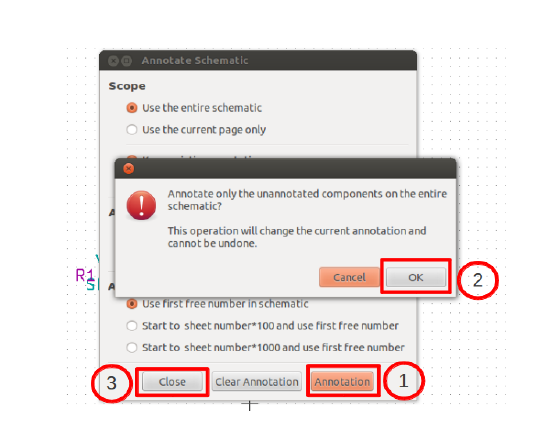
\includegraphics[width=\linewidth]{annotation.png}
  \caption{Annotation}
  \label{annotation}
\end{minipage}%
\begin{minipage}{.5\textwidth}
  \centering
  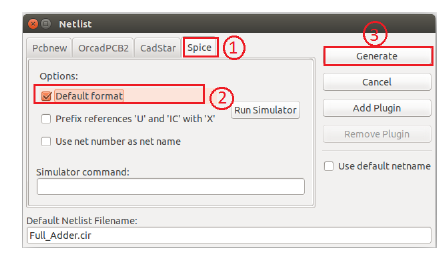
\includegraphics[width=\linewidth]{createnetlist.png}
  \caption{Netlist Generation}
  \label{createnetlist}
\end{minipage}
\end{figure}

\subsection{KiCad to Ngspice conversion}

\paragraph{} To convert KiCad netlist of RC circuit to NgSpice
compatible netlist click on KiCad to Ngspice icon as shown in Figure \ref{kcd2spice}.  Now you can choose the type of analysis, source details, device models ngspice models and subcircuit models.


\begin{figure}[h]
\centering
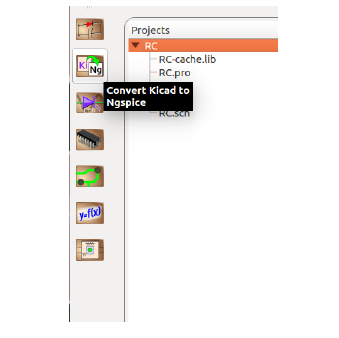
\includegraphics[width=0.5\textwidth, height=4cm]{kcd2spice.png}
\caption{Choose Kicad to Ngspice tool}
\label{kcd2spice}
\end{figure}


\paragraph{Analysis:}Choose AC analysis type and choose Dec scale. Dec sclae allows plotting as in a semilog graph.  Give the values of AC variables as shown in Figure \ref{acanalysis}. Enter the name of your AC source as on the circuit (here v1) and let its frequency be varied from 1Hz to 10kHz with 10 points chosen in each deacade interval of frequency.

\begin{figure}[h]
\centering
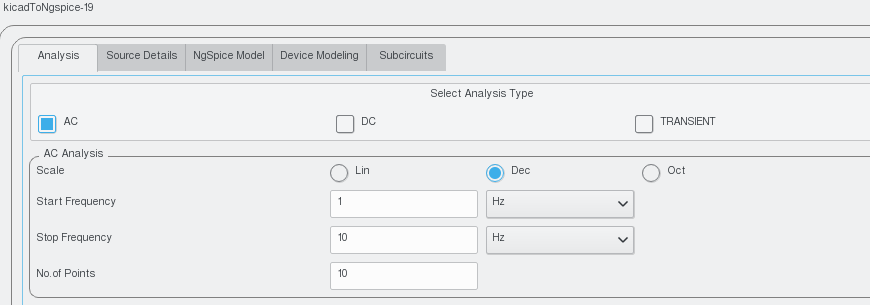
\includegraphics[width=\textwidth, height=4cm]{acanalysis.png}
\caption{Choose AC analysis type and enter the values}
\label{acanalysis}
\end{figure}

\paragraph{Source Details:} Set amplitude as 5 and phase shift as 0.

\paragraph{Ngspice Model:} No Ngspice model to be given.

\paragraph{Device Model:} No Device model to be given.

\paragraph{Subcircuits:} No subcircuits to be given.

\noindent Once these details are provided click on convert button.  Now you are ready to see the simulation results.


\paragraph{}
\subsection{Simulate} To run Ngspice simulation click the simulation icon in the left tool bar. It will open up two windows - ngspice plotting window and python plotting window. Inorder to plot the frequency response characteristics let us use the commands in ngspice plotting window. 

\paragraph{}We need to plot the value of voltage across the AC source Vs the frequency in logarithmic scale as well as the voltage across the resistor Vs the frequency in logarithmic scale. Let us use the command:

\texttt{plot v(Input), v(Output) }

\paragraph{}

This would plot the frequency response characteristics of input and output of the RC high pass filter. The resultant characteristics is shown in the Figure \ref{HPFresponse}. 



The charcteristics of RC low pass filter would be as shown in Figure \ref{LPFresponse}.

\begin{figure}[h]
\centering
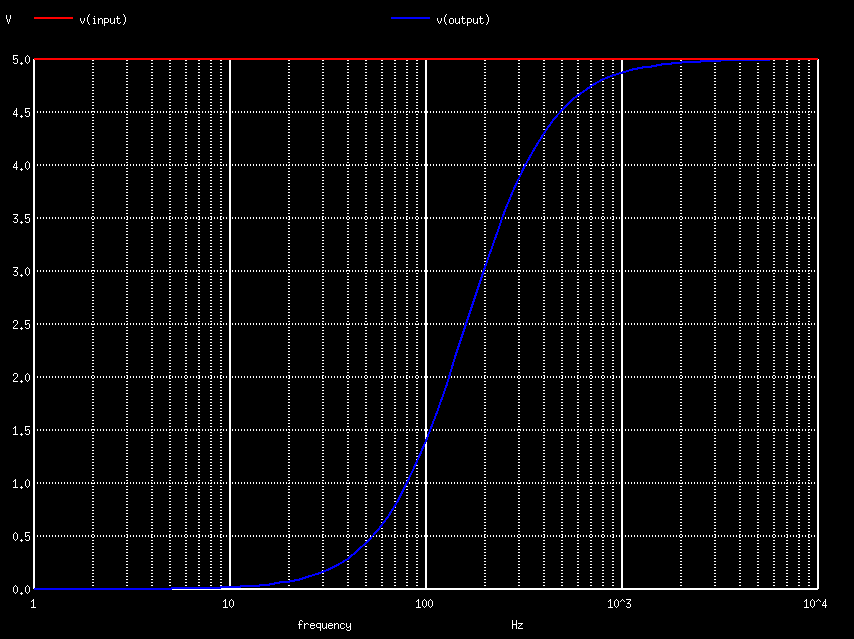
\includegraphics[width=12cm, height=8cm]{LPFresponse.png}
\caption{The frequency response of RC low pass filter}
\label{LPFresponse}
\end{figure}

\begin{figure}[h]
\centering
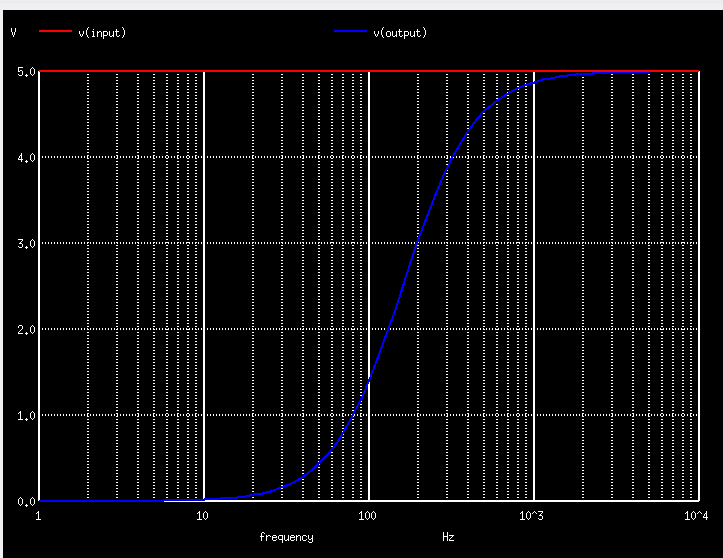
\includegraphics[width=12cm, height=8cm]{HPFresponse.png}
\caption{The frequency response of RC highpass filter}
\label{HPFresponse}
\end{figure}
\section*{RESULT}
The circuit for plotting the frequency response of filter was implemented and simulated.


